\documentclass{beamer}

\usepackage[utf8]{inputenc}
\usepackage[T1]{fontenc}
\usepackage[francais]{babel}
\usepackage{graphics}
\usepackage{graphicx}
\usetheme{MyStyle}

\title{La cryptologie : \\
peut-on réellement cacher des informations ?}
\author{Quentin Stiévenart}
\date{22 juin 2009}
\setbeamertemplate{navigation symbols}{}

\begin{document}

\frame{\titlepage}

\section[Présentation]{}
\frame{\tableofcontents}

\section{Présentation de la cryptologie}
\frame{
  \frametitle{Présentation de la cryptologie}
  \begin{itemize}[<+->]
    \item Cryptographie
      \begin{itemize}[<+->]
        \item Premières techniques au VI\ieme~siècle av. J.-C.
        \item Chiffrer/déchiffrer un message
        \item En constante évolution
        \item Techniques très diverses
        \item Diverses applications
      \end{itemize}
    \item Cryptanalyse
      \begin{itemize}[<+->]
        \item Apparition au IX\ieme~siècle
        \item Casser un message
        \item Nombreux types d'attaque
      \end{itemize}
  \end{itemize}
}

\section{Le chiffre de César}
\subsection{Caractéristiques}
\frame{
  \frametitle{Caractéristiques du chiffre de César}
  \begin{itemize}[<+->]
    \item Chiffrement par substitution simple
    \item Utilisé par César pour transmettre des messages
militaires
    \item Très simple à :
      \begin{itemize}[<+->]
        \item comprendre
        \item mettre en pratique
        \item casser
      \end{itemize}
  \end{itemize}
}

\subsection{Chiffrement}
\frame{
  \frametitle{Chiffrement}

  \begin{itemize}[<+->]
    \item Message à chiffrer : «~message~» avec $k=3$
    \item Chiffrement :  \\
      \begin{tabular}{cccccccl}
        M & E & S & S & A & G & E & $\rightarrow$ message clair \\
        \pause
        N & F & T & T & B & H & F & $\rightarrow k=1$ \\
        \pause
        O & G & U & U & C & I & G & $\rightarrow k=2$ \\
        \pause
        P & H & V & V & D & J & H & $\rightarrow$ message chiffré \\
        \pause
      \end{tabular}
    \item Message chiffré : «~PHVVDJH~»
  \end{itemize}
}

\subsection{Déchiffrement}
\frame{
  \frametitle{Déchiffrement}
  \begin {itemize}[<+->]
    \item Message à déchiffrer : «~PHVDJH~»
    \item Déchiffrement : \\
      \begin{tabular}{cccccccl}
        P & H & V & V & D & J & H & $\rightarrow$ message chiffré \\
        \pause
        O & G & U & U & C & I & G & \\
        \pause
        N & F & T & T & B & H & F & \\
        \pause
        M & E & S & S & A & G & E & $\rightarrow$ message clair \\
        \pause
      \end{tabular}
    \item Message clair : «~message~»
  \end{itemize}
}

\subsection{Cryptanalyse}
\frame{
  \frametitle{Cryptanalyse}
  \begin{itemize}[<+->]
    \item Force brute
    \item Analyse des fréquences
      \pause
      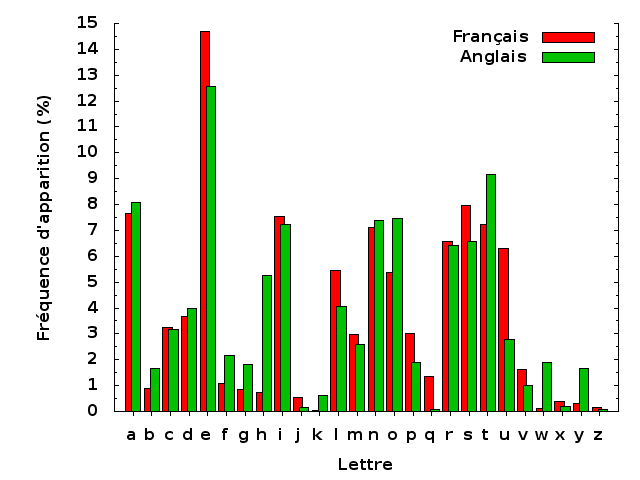
\includegraphics[width=0.9\textwidth]{../texte/plot/Frequences.png}
  \end{itemize}
}

\subsection{Exemple}
\frame{
  \frametitle{Exemple}
    \begin{itemize}[<+->]
      \item Message chiffré : 
        \begin{center}
          BQGFAZDQQXXQYQZFOMOTQDPQEUZRADYMFUAZE
        \end{center}
      \item Fréquences d'apparition : \\
        \begin{center}
        \begin{tabular}{|c|c|}
          \hline
          Lettre & Nombre d'apparition \\
          \hline
          Q & 7 \\
          \hline
          Z & 4 \\
          \hline
          F, D, A, Y & 3 \\
          \hline
          Y, X, U, O, M, E & 2 \\
          \hline
          T, R, P, G, B & 1 \\
          \hline
        \end{tabular}
        \end{center}
    \item Q (17\ieme~lettre de l'alphabet) est sûrement E (5\ieme~lettre)
    \item $k = 17 - 5 = 12$
    \item Déchiffrement avec $k = 12$ :
«~peutonreellementcacherdesinformations~» 
  \end{itemize}
}

\section{Questions}
\frame{
  \frametitle{Questions ?}
}
    
\end{document}

